\chapter{Sums and Asymptotics}\label{chap:asymptotics}

Sums and products arise regularly in the analysis of algorithms,
financial applications, physical problems, and probabilistic systems.
For example, according to Theorem~\ref{sum_to_n_thm},
\begin{equation}\label{sum1n_closedform}
1 + 2 + 3 +\cdots + n = \frac{n(n+1)}{2}.
\end{equation}
Of course, the lefthand sum could be expressed concisely as a
subscripted summation
\[
\sum_{i=1}^n i
\]
but the right hand expression $n(n+1)/2$ is not only concise but also
easier to evaluate.  Furthermore, it more clearly reveals properties
such as the growth rate of the sum.  Expressions like $n(n+1)/2$ that
do not make use of subscripted summations or products---or those handy
but sometimes troublesome sequences of three dots---are called
\term{closed forms}.

Another example is the closed form for a \term{geometric sum}
\begin{equation}\label{geometric-sum-n}
1 + x + x^2 + x^3 + \cdots + x^{n} = \frac{1 - x^{n+1}}{1 - x}
\end{equation}
given in Problem~\ref{CP_geometric_series_induction}.  The sum as
described on the left hand side of~\eqref{geometric-sum-n} involves
$n$ additions and $1 + 2 + \cdots + (n-1) = (n-1)n/2$ multiplications,
but its closed form on the right hand side can be evaluated using fast
exponentiation with at most $2 \log n$ multiplications, a division,
and a couple of subtractions.  Also, the closed form makes the growth
and limiting behavior of the sum much more apparent.

\iffalse

\begin{equation}\label{geometric-sum-n-1}
    \sum_{i = 0}^{n} x^i = \frac{1 - x^{n+1}}{1 - x}.
\end{equation}

In particular, the terms of the sum
\[
    \sum_{j = 0}^{n} x^j = 1 + x + x^2 + x^3 + \cdots + x^{n}
\]
form a \term{geometric series}, which means that the ratio of
consecutive terms is always the same and it is a positive value less
than one.  In this case, the ratio is always~$x$, and $0 < x < 1$
since we assumed that~$p > 0$.  It turns out that there is a nice
closed form expression for any geometric series; namely
\begin{equation}\label{geometric-sum-n-1}
1 + x + x^2 + x^3 + \cdots + x^{n} = \sum_{i = 0}^{n} x^i = \frac{1 - x^{n+1}}{1 - x}.
\end{equation}

For example, we have already encountered the sum $1 + 2 + 4 + \dots +
N$ when counting the number of nodes in a complete binary tree with
$N$ inputs.  Although such a sum can be represented compactly using
the sigma notation
\begin{equation}
    \sum_{i = 0}^{\log N} 2^i,
\end{equation}
it is a lot easier and more helpful to express the sum by
its \term{closed form} value
\[
    2 N - 1.
\]
(it doesn't get much simpler than $2 N - 1$, for example) 

Expressions in closed form are usually easier to evaluate and it is
usually easier to get a feel for their magnitude than expressions
involving large sums and products.\fi

Equations~\eqref{sum1n_closedform} and~\eqref{geometric-sum-n} were
easy to verify by induction, but, as is often the case, the proofs by
induction gave no hint about how these formulas were found in the
first place.  Finding them is part math and part art, which we'll
start examining in this chapter.

Our first motivating example will be the value of a financial
instrument known as an \idx{annuity}.  This value will be a large and
nasty-looking sum.  We will then describe several methods for finding
closed forms for several sorts of sums, including those for annuities.
In some cases, a closed form for a sum may not exist, and so we will
provide a general method for finding closed forms for good upper and
lower bounds on the sum.

The methods we develop for sums will also work for products, since any
product can be converted into a sum by taking its logarithm.  For
instance, later in the chapter we will use this approach to find a
good closed-form approximation to the \emph{\idx{factorial} function}
\[
    n! \eqdef 1 \cdot 2 \cdot 3 \cdots n.
\]

We conclude the chapter with a discussion of asymptotic notation,
especially ``Big Oh'' notation.  Asymptotic notation is often used to
bound the error terms when there is no exact closed form expression
for a sum or product.  It also provides a convenient way to express
the growth rate or order of magnitude of a sum or product.

\section{The Value of an Annuity}\label{annuity_sec}

Would you prefer a million dollars today or \$50,000 a year for the
rest of your life?  On the one hand, instant gratification is nice.
On the other hand, the \emph{total dollars} received at \$50K per year
is much larger if you live long enough.

Formally, this is a question about the value of an annuity.  An
\term{annuity} is a financial instrument that pays out a fixed amount
of money at the beginning of every year for some specified number of
years.  In particular, an $n$-year, $m$-payment annuity pays $m$
dollars at the start of each year for $n$ years.  In some cases, $n$
is finite, but not always.  Examples include lottery payouts, student
loans, and home mortgages.  There are even firms on Wall Street that
specialize in trading annuities.\footnote{Such trading ultimately led
  to the subprime mortgage disaster in 2008--2009.  We'll talk more
  about that in a later chapter.} \iffalse
Chapter~\ref{sec:subprime}\fi

A key question is, ``What is an annuity worth?''  For example,
lotteries often pay out jackpots over many years.  Intuitively,
\$50,000 a year for 20 years ought to be worth less than a million
dollars right now.  If you had all the cash right away, you could
invest it and begin collecting interest.  But what if the choice were
between \$50,000 a year for 20 years and a \emph{half} million
dollars today?  Suddenly, it's not clear which option is better.

\subsection{The Future Value of Money}

In order to answer such questions, we need to know what a dollar paid
out in the future is worth today.  To model this, let's assume that
money can be invested at a fixed annual interest rate $p$.  We'll
assume an 8\% rate\footnote{U.S. interest rates have dropped steadily
  for several years, and ordinary bank deposits now earn around 1.0\%.
  But just a few years ago the rate was 8\%; this rate makes some of
  our examples a little more dramatic.  The rate has been as high as
  17\% in the past thirty years.} for the rest of the discussion, so
$p = 0.08$.

Here is why the interest rate $p$ matters.  Ten dollars invested today
at interest rate $p$ will become $(1+p)\cdot 10 = 10.80$ dollars in a
year, $(1+p)^2\cdot 10 \approx 11.66$ dollars in two years, and so
forth.  Looked at another way, ten dollars paid out a year from now is
only really worth $1/(1+p) \cdot 10 \approx 9.26$ dollars today,
because if we had the \$9.26 today, we could invest it and would have
\$10.00 in a year anyway.  Therefore, $p$ determines the value of
money paid out in the future.

So for an $n$-year, $m$-payment annuity, the first payment of $m$ dollars
is truly worth $m$ dollars.  But the second payment a year later is worth
only $m/(1+p)$ dollars.  Similarly, the third payment is worth
$m/(1+p)^2$, and the $n$-th payment is worth only $m/(1+p)^{n-1}$.  The
total value, $V$, of the annuity is equal to the sum of the payment
values.  This gives:
\begin{align}
  V & = \sum_{i=1}^n \frac{m}{(1+p)^{i-1}}\notag\\
  & = m \cdot \sum_{j=0}^{n-1} \paren{\frac{1}{1+p}}^j
          && \text{(substitute $j = i-1$)}\notag\\
  & = m \cdot \sum_{j=0}^{n-1} x^j
          && \text{(substitute $x = 1/(1+p)$)}.\label{jn-1xsum}
\end{align}

The goal of the preceding substitutions was to get the summation into
the form of a simple geometric sum.  This leads us to an explanation
of a way you could have discovered the closed
form~\eqref{geometric-sum-n} in the first place using the
\term{Perturbation Method}.

\subsection{The Perturbation Method}\label{sec:perturbation}

Given a sum that has a nice structure, it is often useful to
``perturb'' the sum so that we can somehow combine the sum with the
perturbation to get something much simpler.  For example, suppose
\[
    S = 1 + x + x^2 + \dots + x^{n}.
\]
An example of a perturbation would be
\[
    xS = x + x^2 + \dots + x^{n+1}.
\]
The difference between $S$ and~$xS$ is not so great, and so if we were
to subtract~$xS$ from~$S$, there would be massive cancellation:
\[
\begin{series}
      S & = & 1 & + & x & + & x^2 & + & x^3 & + &\cdots & + & x^{n} \cr
    -xS & = &   & - & x & - & x^2 & - & x^3 & - &\cdots & - & x^{n} & - x^{n+1}.\cr
\end{series}
\]
The result of the subtraction is
\[
    S-xS = 1 - x^{n+1}.
\]
Solving for~$S$ gives the desired closed-form expression in
equation~\ref{geometric-sum-n}, namely,
\[
    S = \frac{1 - x^{n+1}}{1 - x}.
\]
We'll see more examples of this method when we introduce
\emph{generating functions} in Chapter~\ref{generating_function_chap}.

\subsection{A Closed Form for the Annuity Value}

Using equation~\ref{geometric-sum-n}, we can derive a simple formula
for~$V$, the \idx{value of an annuity} that pays $m$ dollars at the
start of each year for $n$ years.
\begin{align}
  V & = m \paren{\frac{1 - x^n}{1-x}}
      && \text{(by equations~\ref{jn-1xsum} and~\ref{geometric-sum-n})}\label{Vmfrac1x}\\
  & = m \paren{\frac{1 + p - \paren{1/(1+p)}^{n-1}}{p}}
      && \text{(substituting $x = 1/(1+p)$)}.\label{annval1p}
\end{align}
Equation~\ref{annval1p} is much easier to use than a summation with
dozens of terms.  For example, what is the real value of a winning
lottery ticket that pays \$50,000 per year for 20~years?  Plugging in
$m = \text{\$50,000}$, $n = 20$, and $p = 0.08$ gives $V \approx
\text{\$530,180}$.  So because payments are deferred, the million
dollar lottery is really only worth about a half million dollars!
This is a good trick for the lottery advertisers.

\subsection{Infinite Geometric Series}

We began this chapter by asking whether you would prefer a million
dollars today or \$50,000 a year for the rest of your life.  Of
course, this depends on how long you live, so optimistically assume
that the second option is to receive \$50,000 a year \emph{forever}.
This sounds like infinite money!  But we can compute the value of an
annuity with an infinite number of payments by taking the limit of our
geometric sum in equation~\ref{geometric-sum-n} as $n$ tends to
infinity.
\begin{theorem}\label{th:series}
If $\abs{x} < 1$, then
\[
\sum_{i=0}^\infty x^i = \frac{1}{1-x}.
\]
\end{theorem}

\begin{proof}
\begin{align*}
\sum_{i=0}^\infty x^i
   & \eqdef  \lim_{n \rightarrow \infty} \sum_{i=0}^{n} x^i \\
   & = \lim_{n \rightarrow \infty} \frac{1 - x^{n+1}}{1-x}
        & & \text{(by equation~\ref{geometric-sum-n})}\\
   & = \frac{1}{1-x}.
\end{align*}
The final line follows from the fact that $\lim_{n \rightarrow \infty}
x^{n+1} =0$ when $\abs{x} < 1$.
\end{proof}

In our annuity problem, $x=1/(1+p) < 1$, so Theorem~\ref{th:series}
applies, and we get
\begin{align*}
V & = m \cdot \sum_{j=0}^{\infty} x^j & \text{(by equation~\ref{jn-1xsum})}\\
  &= m\cdot \frac{1}{1-x} & \text{(by Theorem~\ref{th:series})}\\ &=
m\cdot \frac{1 + p}{p} &(x = 1/(1+p)).
\end{align*}
Plugging in $m = \text{\$50,000}$ and $p = 0.08$, we see that the
value~$V$ is only \$675,000.  It seems amazing that a million dollars
today is worth much more than \$50,000 paid every year for eternity!  But
on closer inspection, if we had a million dollars today in the bank
earning 8\% interest, we could take out and spend \$80,000 a year,
\emph{forever}.  So as it turns out, this answer really isn't so
amazing after all.

\subsection{Examples}

Equation~\ref{geometric-sum-n} and Theorem~\ref{th:series} are
incredibly useful in computer science.  \iffalse In fact, we already
used equation~\ref{geometric-sum-n-1} implicitly when we claimed in
Chapter~\ref{chap:digraphs} than an $N$-input complete binary tree has
\[
    1 + 2 + 4 + \dots + N = 2 N - 1
\]
nodes.  \fi

Here are some other common sums that can be put into closed form using
equation~\ref{geometric-sum-n} and Theorem~\ref{th:series}:
\begingroup \openup3pt
\begin{gather}
1 + 1/2 + 1/4 + \cdots = \sum_{i=0}^\infty \paren{\frac{1}{2}}^i %\;\;
= \cfrac{1}{1-(1/2)} = 2 \label{is2} \\ 0.99999\dots = 0.9
\sum_{i=0}^{\infty} \paren{\frac{1}{10}}^i = 0.9
\paren{\cfrac{1}{1-1/10}} = 0.9 \paren{\cfrac{10}{9}} = 1 \label{is1}
\\ 1 - 1/2 + 1/4 - \cdots = \sum_{i=0}^\infty \paren{\frac{-1}{2}}^i =
\cfrac{1}{1-(-1/2)} = \frac{2}{3} \label{is23} \\ 1 + 2 + 4 + \cdots +
2^{n-1} = \sum_{i=0}^{n-1} 2^i = \cfrac{1 - 2^n}{1 - 2} = 2^n -
1 \label{is2n1} \\ 1 + 3 + 9 + \cdots + 3^{n-1} = \sum_{i=0}^{n-1} 3^i
= \cfrac{1 - 3^n}{1 - 3} = \cfrac{3^n - 1}{2} \label{is3n1}
\end{gather}
\endgroup

If the terms in a geometric sum grow smaller, as in
equation~\ref{is2}, then the sum is said to be \emph{geometrically
  decreasing}.  If the terms in a geometric sum grow progressively
larger, as in equations \ref{is2n1} and~\ref{is3n1}, then the sum is
said to be \emph{geometrically increasing}.  In either case, the sum
is usually approximately equal to the term in the sum with the
greatest absolute value.  For example, in equations \ref{is2}
and~\ref{is23}, the largest term is equal to 1 and the sums are 2 and
2/3, both relatively close to~1.  In equation~\ref{is2n1}, the sum is
about twice the largest term.  In equation~\ref{is3n1}, the largest
term is $3^{n-1}$ and the sum is $(3^n-1)/2$, which is only about a
factor of $1.5$ greater.  You can see why this rule of thumb works by
looking carefully at equation~\ref{geometric-sum-n} and
Theorem~\ref{th:series}.

\subsection{Variations of Geometric Sums}\label{variant_sum_sec}

We now know all about geometric sums---if you have one, life is easy.
But in practice one often encounters sums that cannot be transformed
by simple variable substitutions to the form $\sum x^i$.

A non-obvious but useful way to obtain new summation formulas from
old ones is by differentiating or integrating with respect to $x$.  As
an example, consider the following sum:
\[
\sum_{i=1}^{n-1} i x^i = x + 2 x^2 + 3 x^3 + \cdots + (n - 1) x^{n -
  1}
\]
This is not a geometric sum.  The ratio between successive terms
is not fixed, and so our formula for the sum of a geometric sum cannot
be directly applied.  But differentiating
equation~\ref{geometric-sum-n} leads
to:
\begin{equation}\label{eqn:9A}
\frac{d}{dx} \paren{ \sum_{i = 0}^{n - 1} x^i }
   = \frac{d}{dx} \paren{ \frac{1 - x^n}{1 - x} }.
\end{equation}
The left-hand side of equation~\ref{eqn:9A} is simply
\[
\sum_{i = 0}^{n - 1} \frac{d}{dx} (x^i)
    = \sum_{i = 0}^{n - 1} i x^{i - 1}.
\]
The right-hand side of equation~\ref{eqn:9A} is
\begin{align*}
\frac{ -n x^{n - 1} (1 - x) - (-1) (1 - x^n) }{ (1 - x)^2 }
    &= \frac{ -n x^{n - 1} + n x^n + 1 - x^n }{ (1 - x)^2 } \\
    &= \frac{1 - n x^{n - 1} + (n - 1) x^n}{ (1 - x)^2 }.
\end{align*}
Hence, equation~\ref{eqn:9A} means that
\[
\sum_{i = 0}^{n - 1} i x^{i - 1}
    = \frac{1 - n x^{n - 1} + (n - 1) x^n}{ (1 - x)^2 }.
\]
Incidentally, Problem~\ref{CP_neat_trick_for_geometric_sum} shows how
the perturbation method could also be applied to derive this formula.

Often, differentiating or integrating messes up the exponent of $x$ in
every term.  In this case, we now have a formula for a sum of the form
$\sum i x^{i-1}$, but we want a formula for the series $\sum i x^i$.
The solution is simple: multiply by $x$.  This gives:
\begin{equation}\label{eqn:sumixi}
    \sum_{i=1}^{n - 1} i x^i = \frac{ x - n x^n + (n - 1) x^{n+1}}{(1 - x)^2}
\end{equation}
and we have the desired closed-form expression for our sum. It seems a
little complicated, but it's easier to work with than the sum.

\begin{editingnotes}
%footnote

Since we could easily have made a mistake in the calculation, it is
always a good idea to go back and validate a formula obtained this way
with a proof by induction.
\end{editingnotes}


Notice that if $\abs{x} < 1$, then this series converges to a finite
value even if there are infinitely many terms.  Taking the limit of
equation~\ref{eqn:sumixi} as $n$ tends to infinity gives the following
theorem:
\begin{theorem}\label{th:inf_ixi}
If $\abs{x} < 1$, then
\begin{equation}\label{eqn:inf_ixi}
    \sum_{i=1}^\infty i x^i = \frac{x}{(1-x)^2}.
\end{equation}
\end{theorem}

As a consequence, suppose that there is an annuity that pays
$im$~dollars at the end of each year~$i$, forever.  For example,
if $m = \text{\$50,000}$, then the payouts are \$50,000 and then
\$100,000 and then \$150,000 and so on.  It is hard to believe
that the value of this annuity is finite!  But we can use
Theorem~\ref{th:inf_ixi} to compute the value:
\begin{align*}
V & = \sum_{i=1}^\infty \frac{im}{(1+p)^i} \\
  & = m \cdot \frac{1/(1+p)}{(1 - \frac{1}{1+p})^2} \\
  & = m \cdot \frac{1+p}{p^2}.
\end{align*}
The second line follows by an application of Theorem~\ref{th:inf_ixi}.
The third line is obtained by multiplying the numerator and
denominator by $(1+p)^2$.

For example, if $m = \text{\$50,000}$, and $p = 0.08$ as usual, then
the value of the annuity is $V = \text{\$8,437,500}$.  Even though the
payments increase every year, the increase is only additive with time;
by contrast, dollars paid out in the future decrease in value
exponentially with time.  The geometric decrease swamps out the
additive increase.  Payments in the distant future are almost
worthless, so the value of the annuity is finite.

The important thing to remember is the trick of taking the derivative
(or integral) of a summation formula.  Of course, this technique
requires one to compute nasty derivatives correctly, but this is at
least theoretically possible!

\begin{problems}
\classproblems
\pinput{PS_mixing_water_and_wine}
\pinput{CP_neat_trick_for_geometric_sum}
\pinput{CP_Sammy_the_shark}

\homeworkproblems
\pinput{PS_MIT_Harvard_degree_value}
\pinput{PS_credit_union}

\end{problems}

\section{Sums of Powers}\label{sec:sum_powers}

In Chapter~\ref{induction_chap}, we verified the formula~\eqref{sum1n_closedform},
\iffalse
\begin{equation}\label{eqn:G26}
    \sum_{i = 1}^n i = \frac{n (n + 1)}{2}.
\end{equation}\fi
but the source of this formula is still a mystery.  Sure, we can prove
that it's true by using well ordering or induction, but where did the
expression on the right come from in the first place?  Even more
inexplicable is the closed form expression for the sum of consecutive
squares:
\begin{equation}\label{eqn:G27}
    \sum_{i = 1}^n i^2 = \frac{(2n+1) (n+1) n}{6}.
\end{equation}

It turns out that there is a way to derive these expressions, but
before we explain it, we thought it would be fun---OK, our definition
of ``fun'' may be different than yours---to show you how Gauss is
supposed to have proved equation~\ref{sum1n_closedform} when he was a
young boy.

\iffalse
\footnote{We suspect that Gauss was probably not an ordinary boy.}
\fi

Gauss's idea is related to the perturbation method we used in
Section~\ref{sec:perturbation}.  Let
\[
    S = \sum_{i = 1}^n i.
\]
Then we can write the sum in two orders:
\[
    \begin{series}
        S & = & 1 & + & 2       & + & \dots & + & (n - 1) & + & n,\cr
        S & = & n & + & (n - 1) & + & \dots & + & 2       & + & 1.
    \end{series}
\]
Adding these two equations gives
\begin{align*}
    2S  & = (n + 1) + (n + 1) + \dots + (n + 1) + (n + 1) \\
        & = n (n + 1).
\end{align*}
Hence,
\[
    S = \frac{n (n + 1)}{2}.
\]
Not bad for a young child---Gauss showed some potential\dots.

Unfortunately, the same trick does not work for summing consecutive
squares.  However, we can observe that the result might be a
third-degree polynomial in~$n$, since the sum contains $n$~terms that
average out to a value that grows quadratically in~$n$.  So we might
guess that
\[
    \sum_{i=1}^n i^2 = an^3 + bn^2 + cn + d.
\]
If our guess is correct, then we can determine the parameters $a$,
$b$, $c$, and $d$ by plugging in a few values for $n$.  Each such
value gives a linear equation in $a$, $b$, $c$, and $d$.  If we plug
in enough values, we may get a linear system with a unique solution.
Applying this method to our example gives:
\begin{align*}
n = 0 & \qimplies  0 = d \\
n = 1 & \qimplies  1 = a + b + c + d \\
n = 2 & \qimplies  5 = 8a + 4b + 2c + d \\
n = 3 & \qimplies  14 = 27a + 9b + 3c + d.
\end{align*}
Solving this system gives the solution $a = 1/3$, $b = 1/2$, $c =
1/6$, $d = 0$.  Therefore, \emph{if} our initial guess at the form of
the solution was correct, then the summation is equal to $n^3/3 +
n^2/2 + n/6$, which matches equation~\ref{eqn:G27}.

The point is that if the desired formula turns out to be a polynomial,
then once you get an estimate of the \emph{degree} of the polynomial,
all the coefficients of the polynomial can be found automatically.

\textbf{Be careful!}  This method lets you discover formulas, but it
doesn't guarantee they are right!  After obtaining a formula by this
method, it's important to go back and \emph{prove} it by induction
or some other method.  If the initial guess at the solution was
not of the right form, then the resulting formula will be completely
wrong!  A later chapter will describe
%~\ref{generating_function_chap}
a method based on generating functions that does not require any
guessing at all.

\begin{problems}
\classproblems
\pinput{CP_sum_dif_frac}

\end{problems}

\section{Approximating Sums}\label{sec:integral_method}

Unfortunately, it is not always possible to find a closed-form
expression for a sum.  For example, no closed form is known for
\[
    S = \sum_{i = 1}^n \sqrt{i}.
\]

In such cases, we need to resort to approximations for~$S$ if we want
to have a closed form.  The good news is that there is a general
method to find closed-form upper and lower bounds that works well for
many sums.  Even better, the method is simple and easy to remember.
It works by replacing the sum by an integral and then adding either
the first or last term in the sum.

\begin{definition}\label{weakly_increasing_function_def}
A function~$f: \reals^+ \to \reals^+$
is \term{strictly increasing} when
\[
x < y \QIMPLIES f(x) < f(y),
\]
and it is \term{weakly increasing}\footnote{Weakly increasing
  functions are usually called \term{nondecreasing} functions.  We
  will avoid this terminology to prevent confusion between being a
  nondecreasing function and the much weaker property
  of \emph{not} being a decreasing function.} when
\[
x < y \QIMPLIES f(x) \le f(y).
\]

Similarly, $f$ is \term{strictly decreasing} when
\[
x < y \QIMPLIES f(x) > f(y),
\]
and it is \term{weakly decreasing}\footnote{Weakly decreasing
  functions are usually called \term{nonincreasing}.}  when
\[
x < y \QIMPLIES f(x) \ge f(y).
\]
\end{definition}

For example, $2^x$ and $\sqrt{x}$ are strictly increasing functions,
while $\max\{x,2\}$ and $\ceil{x}$ are weakly increasing functions.  The
functions $1/x$ and $2^{-x}$ are strictly decreasing, while $\min\{1/x,
  1/2\}$ and $\floor{1/x}$ are weakly decreasing.

\begin{theorem}\label{weak_increasing_sum_bounds}  %{thm:9G3}
Let $f: \reals^+ \to \reals^+$ be a weakly increasing function.
Define
\begin{equation}\label{Sdefsumf}
    S \eqdef \sum_{i = 1}^n f(i)
\end{equation}
and
\[
    I \eqdef \int_1^n f(x)\, dx.
\]
Then
\begin{equation}\label{If1lS}
    I + f(1) \le S \le I + f(n).
\end{equation}
Similarly, if $f$ is weakly decreasing, then
\[
    I + f(n) \le S \le I + f(1).
\]
\end{theorem}

\begin{proof}
Suppose $f: \reals^+ \to \reals^+$ is weakly increasing.  The value of
the sum $S$ in~\eqref{Sdefsumf} is the sum of the areas of $n$
unit-width rectangles of heights $f(1),f(2),\dots, f(n)$.  This area
of these rectangles is shown shaded in Figure~\ref{fig:9G4}.

\begin{figure}

\graphic{Fig_G4}

\caption{The area of the $i$th rectangle is~$f(i)$.  The shaded region
has area $\sum_{i = 1}^n f(i)$.}

\label{fig:9G4}

\end{figure}

The value of
\[
    I = \int_1^n f(x) \, dx
\]
is the shaded area under the curve of~$f(x)$ from 1 to~$n$ shown in
Figure~\ref{fig:9G5}.

\begin{figure}

\graphic{Fig_G5}

\caption{The shaded area under the curve of~$f(x)$ from 1 to~$n$
  (shown in bold) is $I = \int_1^n f(x)\, dx$.}

\label{fig:9G5}

\end{figure}

Comparing the shaded regions in Figures \ref{fig:9G4}
and~\ref{fig:9G5} shows that $S$ is at least $I$~plus the area of the
leftmost rectangle.  Hence,
\begin{equation}\label{eqn:9G7}
    S \ge I + f(1)
\end{equation}
This is the lower bound for~$S$ given in~\eqref{If1lS}.

To derive the upper bound for~$S$ given in~\eqref{If1lS}, we shift the
curve of~$f(x)$ from 1 to~$n$ one unit to the left as shown in
Figure~\ref{fig:9G6}.
\iffalse This is the same as the curve~$f(x + 1)$ from 0 to~$n - 1$
and it has the same area~$I$.  \fi

\begin{figure}

\graphic{Fig_G6}

\caption{This curve is the same as the curve in Figure~\ref{fig:9G5}
  shifted left by~1.}

\label{fig:9G6}

\end{figure}

Comparing the shaded regions in Figures \ref{fig:9G4}
and~\ref{fig:9G6} shows that $S$~is at most $I$~plus the area of the
rightmost rectangle.  That is,
%\begin{equation}\label{eqn:9G8}
\[
S \le I + f(n),
\]
%\end{equation}
which is the upper bound for~$S$ given in~\eqref{If1lS}.

The very similar argument for the weakly decreasing case is left to
Problem~\ref{CP_sum_bound_by_integral}.

\end{proof}

\iffalse

\begin{figure}

\subfloat[]{\graphic{Fig_G9-a}}

\subfloat[]{\graphic{Fig_G9-b}}

\subfloat[]{\graphic{Fig_G9-c}}

\caption{The area of the shaded region in~(a) is $S = \sum_{i = 1}^n
  f(i)$.  The area in the shaded regions in (b) and~(c) is $I =
  \int_1^n f(x)\,dx$.}

\label{fig:9G9}

\end{figure}
\fi

Theorem~\ref{weak_increasing_sum_bounds} provides good bounds for most sums.  At worst,
the bounds will be off by the largest term in the sum.  For example,
we can use Theorem~\ref{weak_increasing_sum_bounds} to bound the sum
\[
    S = \sum_{i = 1}^n \sqrt{i}
\]
as follows.

We begin by computing
\begin{align*}
    I   &= \int_1^n \sqrt{x} \, dx \\
        &= \left. \frac{x^{3/2}}{3/2} \; \right|_1^n \\
        &= \frac{2}{3} (n^{3/2} - 1).
\end{align*}
We then apply Theorem~\ref{weak_increasing_sum_bounds} to conclude that
\[
    \frac{2}{3} (n^{3/2} - 1) + 1
    \; \le \; S
    \; \le \; \frac{2}{3} (n^{3/2} - 1) + \sqrt{n}
\]
and thus that
\[
    \frac{2}{3} n^{3/2} + \frac{1}{3}
    \; \le \; S
    \; \le \; \frac{2}{3} n^{3/2} + \sqrt{n} - \frac{2}{3}.
\]
In other words, the sum is very close to~$\frac{2}{3} n^{3/2}$.  We'll
define several ways that one thing can be ``very close to'' something
else at the end of this chapter.

As a first application of Theorem~\ref{weak_increasing_sum_bounds}, we
explain in the next section how it helps in resolving a classic
paradox in structural engineering.

\begin{problems}
\practiceproblems
\pinput{TP_The_Integral_Method}

\classproblems
\pinput{CP_integral_sum_asymptotic}

\examproblems
\pinput{MQ_integral_method}

\homeworkproblems
\pinput{CP_sum_bound_by_integral}
\pinput{PS_tight_bounds_with_integral_method}

\end{problems}


\section{Hanging Out Over the Edge}\label{book_stacking_sec}
\index{Book Stacking Problem}
Suppose you have a bunch of books and you want to stack them up, one
on top of another in some off-center way, so the top book sticks out
past books below it without falling over.  If you moved the stack to
the edge of a table, how far past the edge of the table do you think
you could get the top book to go?  Could the top book stick out
completely beyond the edge of table?  You're not supposed to use glue
or any other support to hold the stack in place.

Most people's first response to the Book Stacking Problem---sometimes also their
second and third responses---is ``No, the top book will never get
completely past the edge of the table.''  But in fact, you can get the
top book to stick out as far as you want: one booklength, two
booklengths, any number of booklengths!

\subsection{Formalizing the Problem}

We'll approach this problem recursively.  How far past the end of the
table can we get one book to stick out?  It won't tip as long as its
center of mass is over the table, so we can get it to stick out half its
length, as shown in Figure~\ref{one-stable-book}.

\begin{figure}[htbp]
\centerline{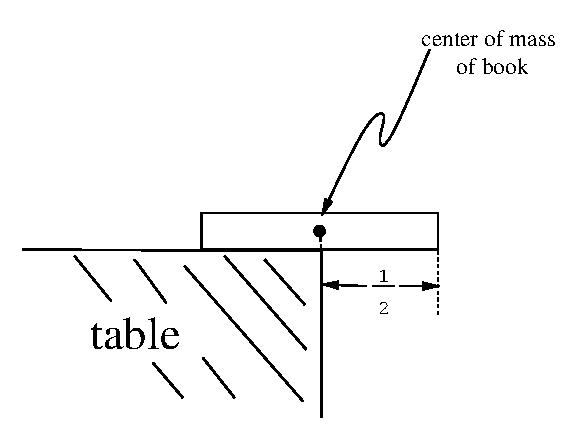
\includegraphics[width=.60\textwidth]{figures/drafts/bookstack-3}}
\caption{One book can overhang half a book length.}
\label{one-stable-book}
\end{figure}

Now suppose we have a stack of books that will not tip over if the
bottom book rests on the table---call that a \emph{stable stack}.
Let's define the \emph{overhang} of a stable stack to be the
horizontal distance from the center of mass of the stack to the
furthest edge of the top book.  So the overhang is purely a property
of the stack, regardless of its placement on the table.  If we place
the center of mass of the stable stack at the edge of the table as in
Figure~\ref{overhang}, the overhang is how far we can get the top book
in the stack to stick out past the edge.

\begin{figure}
\centerline{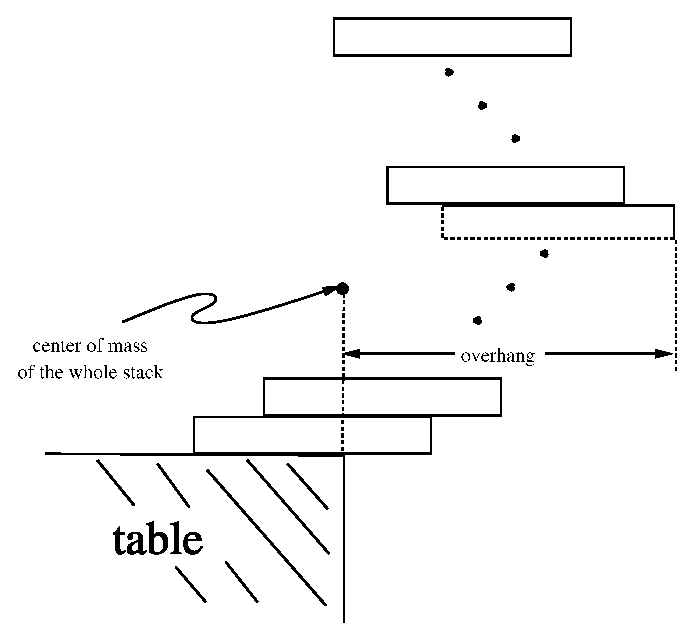
\includegraphics[width=.6\textwidth]{figures/drafts/bookstack-2}}
%\centerline{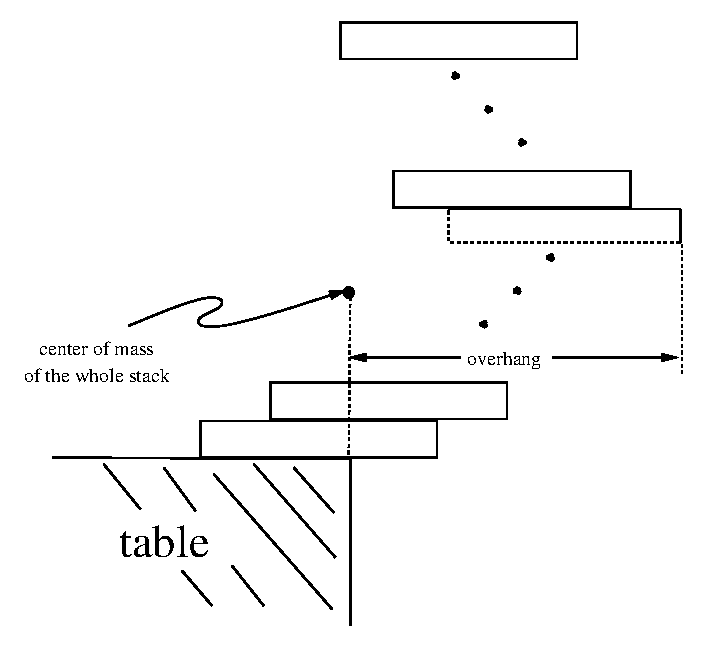
\psfig{file=figures/bookstack-2.ps,width=.4\textwidth}}
\caption{Overhanging the edge of the table.}
\label{overhang}
\end{figure}

In general, a stack of $n$~books will be stable if and only if the
center of mass of the top $i$~books sits over the $(i + 1)$st book
for $i = 1$, 2, \dots, $n - 1$.

So we want a formula for the maximum possible overhang, $B_n$, achievable
with a stable stack of $n$~books.

We've already observed that the overhang of one book is~1/2 a book
length.  That is,
\[
    B_1 = \frac{1}{2}.
\]

Now suppose we have a stable stack of $n+1$ books with maximum overhang.
If the overhang of the $n$ books on top of the bottom book was not
maximum, we could get a book to stick out further by replacing the top
stack with a stack of $n$ books with larger overhang.  So the maximum
overhang, $B_{n+1}$, of a stack of $n+1$ books is obtained by placing a
maximum overhang stable stack of $n$ books on top of the bottom book.  And
we get the biggest overhang for the stack of $n+1$ books by placing the
center of mass of the $n$ books right over the edge of the bottom book as
in Figure~\ref{Bn1}.

So we know where to place the $n+1$st book to get maximum overhang.
In fact, the reasoning above actually shows that this way of stacking
$n+1$ books is the \emph{unique} way to build a stable stack where the
top book extends as far as possible.  All we have to do is
calculate what this extension is.  

The simplest way to do that is to let the center of mass of the top
$n$ books be the origin.  That way the horizontal coordinate of the
center of mass of the whole stack of $n+1$ books will equal the
increase in the overhang.  But now the center of mass of the bottom
book has horizontal coordinate $1/2$, so the horizontal coordinate of
center of mass of the whole stack of $n+1$ books is
\[
\frac{0 \cdot n + (1/2) \cdot 1}{n+1} = \frac{1}{2(n +1)}.
\]

In other words, 
\begin{equation}\label{eqBn}
    B_{n+1} = B_n + \frac{1}{2(n+1)},
\end{equation}
as shown in Figure~\ref{Bn1}.

\begin{figure}
\centerline{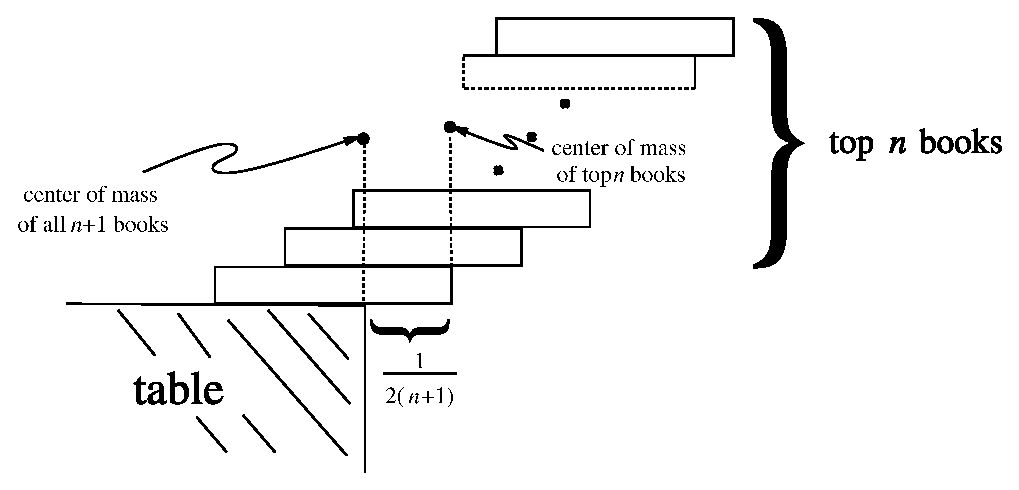
\includegraphics[width=.80\textwidth]{figures/drafts/bookstack-5}}
%\centerline{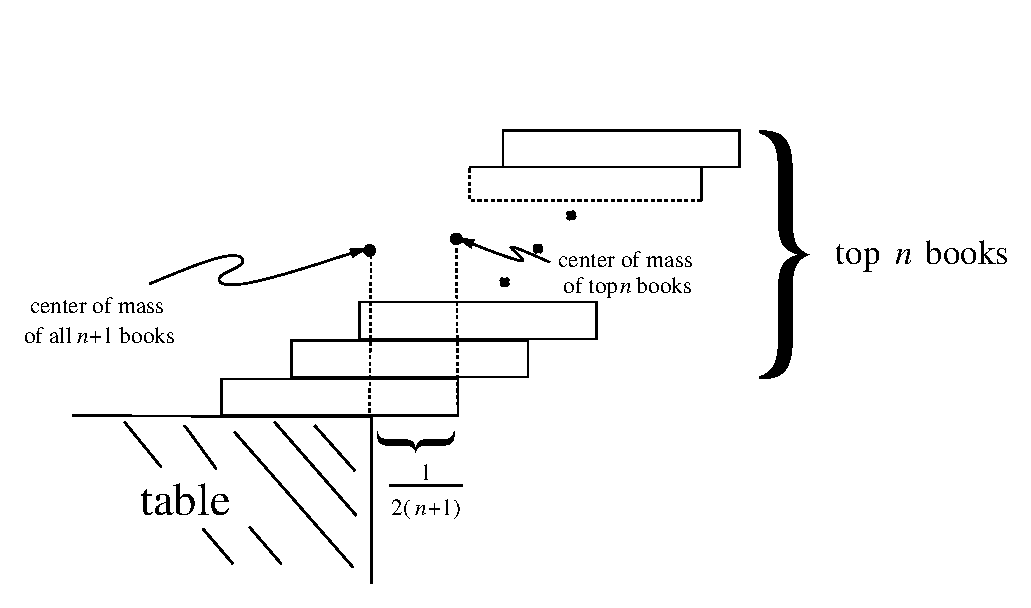
\psfig{file=figures/bookstack-5.ps,width=.80\textwidth}}
\caption{Additional overhang with $n+1$ books.}
\label{Bn1}
\end{figure}

Expanding equation~(\ref{eqBn}), we have
\begin{align}
B_{n+1} & = B_{n-1} + \frac{1}{2n} + \frac{1}{2(n+1)}\notag\\
        & = B_1 + \frac{1}{2 \cdot 2} + \cdots + \frac{1}{2n} +
            \frac{1}{2(n+1)}\notag\\
        & = \frac{1}{2}\sum_{i=1}^{n+1} \frac{1}{i}.\label{Bn+1sum}
\end{align}

So our next task is to examine the behavior of $B_n$ as $n$ grows.

\subsection{Harmonic Numbers}

\begin{definition}
The $n$th \term{harmonic number}, $H_n$, is
\[
H_n \eqdef \sum_{i=1}^n \frac{1}{i}.
\]
\end{definition}
So~\eqref{Bn+1sum} means that
\[
B_n = \frac{H_n}{2}.
\]

The first few harmonic numbers are easy to compute.  For example, $H_4 = 1
+ \frac{1}{2} + \frac{1}{3} + \frac{1}{4} = \frac{25}{12} > 2$.  The fact that
$H_4$ is greater than 2 has special significance: it implies that the
total extension of a 4-book stack is greater than one full book!  This is
the situation shown in Figure~\ref{fig:optstack}.

\begin{figure}[htbp]
\centerline{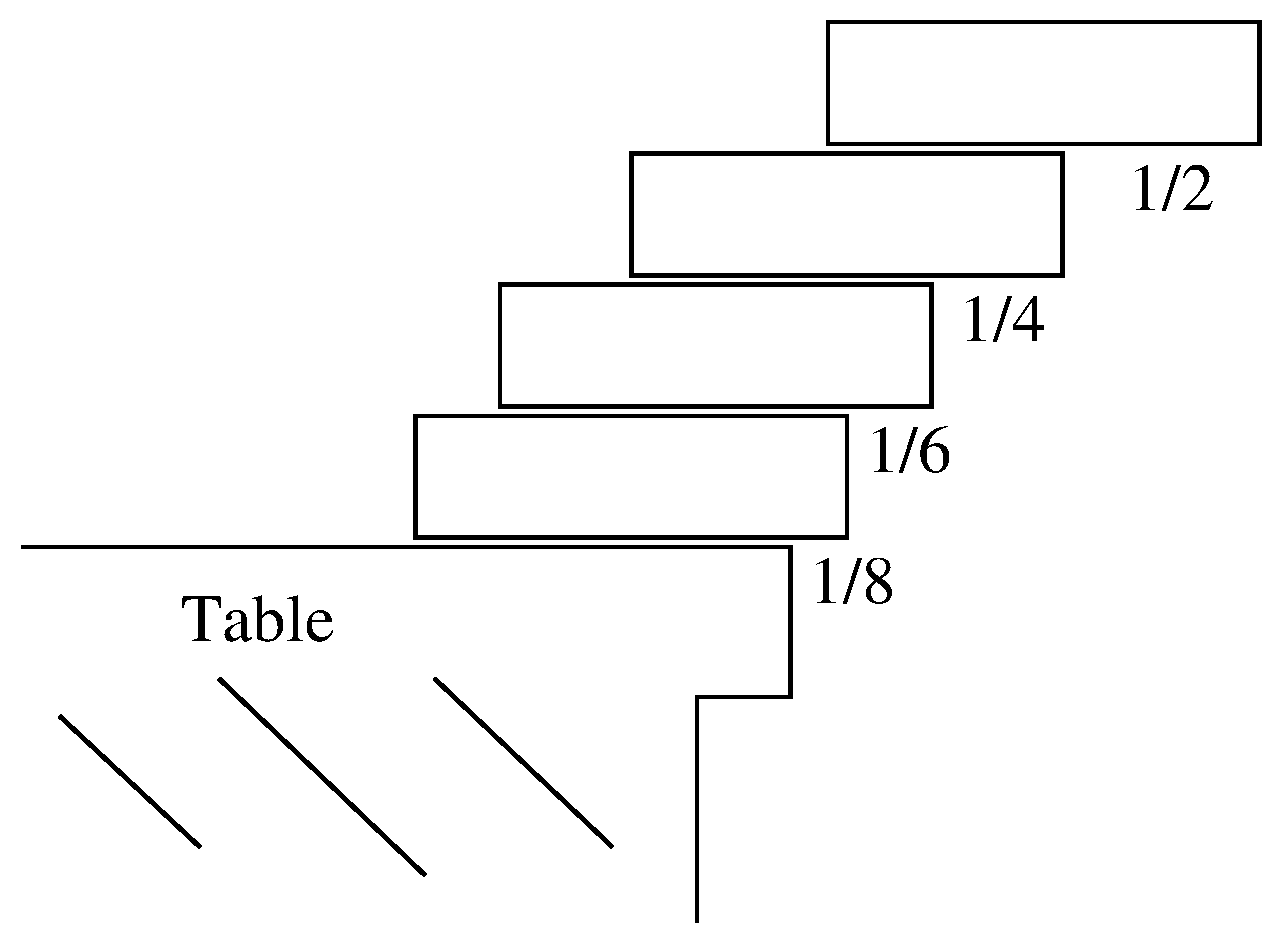
\includegraphics[height=1.5in]{figures/drafts/optstack}}
\caption{Stack of four books with maximum overhang.}
\label{fig:optstack}
\end{figure}

There is good news and bad news about harmonic numbers.  The bad news
is that there is no known closed-form expression for the harmonic
numbers.  The good news is that we can use
Theorem~\ref{weak_increasing_sum_bounds} to get close upper and lower
bounds on~$H_n$.  In particular, since
\begin{align*}
\int_1^n \frac{1}{x} \, dx
    = \ln(x) \; \Bigr|_1^n %\\
    = \ln(n),
\end{align*}
Theorem~\ref{weak_increasing_sum_bounds} means that
\begin{equation}\label{eqn:9G30}
    \ln(n) + \frac{1}{n} \le H_n \le \ln(n) + 1.
\end{equation}
In other words, the $n$th harmonic number is very close to~$\ln(n)$.

Because the harmonic numbers frequently arise in practice,
mathematicians have worked hard to get even better approximations for
them.  In fact, it is now known that
\begin{equation}\label{eqn:9K2}
    H_n = \ln(n) + \gamma + \frac{1}{2n} + \frac{1}{12n^2} +
        \frac{\epsilon(n)}{120n^4}
\end{equation}
Here $\gamma$ is a value $0.577215664\dots$ called \term{Euler's
  constant}, and $\epsilon(n)$ is between 0 and 1 for all $n$.  We
will not prove this formula.

We are now finally done with our analysis of the book stacking
problem.  Plugging the value of~$H_n$ into~\eqref{Bn+1sum}, we
find that the maximum overhang for $n$~books is very close
to~$1/2\ln(n)$.  Since $\ln(n)$ grows to infinity as $n$~increases,
this means that if we are given enough books \begin{editingnotes}
(in theory anyway)
\end{editingnotes},
we can get a book to hang out arbitrarily far over the edge of the table.
Of course, the number of books we need will grow as an exponential
function of the overhang; it will take 227~books just to achieve an
overhang of~3, never mind an overhang of~100.

\subsubsection{Extending Further Past the End of the Table}
The overhang we analyzed above was the furthest out the \emph{top}
book could extend past the table.  This leaves open the question
of if there is some better way to build a stable stack where some book
other than the top stuck out furthest.  For example,
Figure~\ref{lab:bottom-book-furthest} shows a stable stack of two
books where the bottom book extends further out than the top book.
Moreover, the bottom book extends 3/4 of a book length past the end of
the table, which is the same as the maximum overhang for the top book
in a two book stack.

\begin{figure}
\subfloat[]{\graphic{Fig_G20-a}}
\qquad
\subfloat[]{\graphic{Fig_G20-b}}

\caption{Figure (a) shows a stable stack of two books where the
  bottom book extends the same amount past the end of the table as
  the maximum overhang two-book stack shown in Figure (b).}
\label{lab:bottom-book-furthest}
\end{figure}

Since the two book arrangement in
Figure~\ref{lab:bottom-book-furthest}(a) ties the maximum overhang
stack in Figure~\ref{lab:bottom-book-furthest}(b), we could take the
unique stable stack of $n$ books where the top book extends furthest,
and switch the top two books to look like
Figure~\ref{lab:bottom-book-furthest}(a).  This would give a stable
stack of $n$ books where the second from the top book extends the same
maximum overhang distance.  So for $n>1$, there are at least two ways
of building a stable stack of $n$ books which both extend the maximum
overhang distance---one way where the top book is furthest out, and
another way where the second from the top book is furthest out.

It turns out that there is no way to beat these two ways of making
stable stacks.  In fact, it's not too hard to show that these are the
\emph{only} two ways to get a stable stack of books that achieves
maximum overhang.
\begin{editingnotes}
(see Problem~\ref{PS_optimal_overhang}).
\end{editingnotes}

But there is more to the story.  All our reasoning above was about
stacks in which \emph{one} book rests on another.  It turns out that
by building structures in which more than one book rests on top of
another book---think of an inverted pyramid---it is possible to get a
stack of $n$ books to extend proportional to $\sqrt[3]{n}$---much more
than $\ln n$---book lengths without falling over.
See~\cite{Paterson09},
\href{http://mathdl.maa.org/mathDL/22/?pa=content&sa=viewDocument&nodeId=3623&pf=1}
     {\emph{Maximum Overhang}}.


\subsection{Asymptotic Equality}\label{sec:asymptotic_equality}

For cases like equation~\ref{eqn:9K2} where we understand the growth
of a function like~$H_n$ up to some (unimportant) error terms, we use
a special notation,~$\sim$, to denote the leading term of the
function.  For example, we say that $H_n \sim \ln(n)$ to indicate that
the leading term of $H_n$ is $\ln(n)$.  More precisely:
\begin{definition}\label{def:sim}
  For functions $f,g: \reals \to \reals$, we say $f$ is%
\index{asymptotic notation!asymptotic equality|textbf}
\emph{asymptotically equal} to $g$, in symbols,
\[
f(x) \sim g(x)
\]
iff
\[
\lim_{x \rightarrow \infty} f(x)/g(x) = 1.
\]
\end{definition}

Although it is tempting to write $H_n \sim \ln(n) + \gamma$ to indicate
the two leading terms, this is not really right.  According to
Definition~\ref{def:sim}, $H_n \sim \ln(n) + c$ where $c$ is \emph{any
  constant}.  The correct way to indicate that $\gamma$ is the
second-largest term is $H_n - \ln(n) \sim \gamma$.

The reason that the $\sim$ notation is useful is that often we do not care
about lower order terms.  For example, if $n = 100$, then we can compute
$H(n)$ to great precision using only the two leading terms:
\[
\abs{H_n - \ln(n) - \gamma} \leq \abs{\frac{1}{200} - \frac{1}{120000} +
\frac{1}{120 \cdot 100^4}} < \frac{1}{200}.
\]

We will spend a lot more time talking about asymptotic notation at the
end of the chapter.  But for now, let's get back to using sums.

\begin{problems}
\classproblems
\pinput{CP_holy_grail}
\pinput{CP_harmonic_number_divergence}

\homeworkproblems
\pinput{PS_bug_on_rug_harmonic_number}
\begin{editingnotes}
\pinput{PS_optimal_overhang}
\end{editingnotes}

\examproblems
\pinput{MQ_Summation}

\end{problems}

\section{Products}\label{sec:closed_products}

We've covered several techniques for finding closed forms for sums but
no methods for dealing with products.  Fortunately, we do not need to
develop an entirely new set of tools when we encounter a product such
as
\begin{equation}\label{eqn:9P1}
    n! \eqdef \prod_{i = 1}^n i.
\end{equation}
That's because we can convert any product into a sum by taking a
logarithm.  For example, if
\[
    P = \prod_{i  = 1}^n f(i),
\]
then
\[
    \ln(P) = \sum_{i = 1}^n \ln(f(i)).
\]
We can then apply our summing tools to find a closed form (or
approximate closed form) for~$\ln(P)$ and then exponentiate at the end
to undo the logarithm.

For example, let's see how this works for the \idx{factorial}
function~$n!$.  We start by taking the logarithm:
\begin{align*}
\ln (n!)
       & =  \ln(1 \cdot 2 \cdot 3 \cdots (n-1) \cdot n) \\
       & =  \ln(1) + \ln(2) + \ln(3) + \cdots + \ln(n-1) + \ln(n) \\
       & =  \sum_{i=1}^n \ln(i).
\end{align*}

Unfortunately, no closed form for this sum is known.  However, we can
apply Theorem~\ref{weak_increasing_sum_bounds} to find good
closed-form bounds on the sum.  To do this, we first compute
\begin{align*}
\int_1^n \ln(x) \, dx
    &= x \ln(x) - x \Bigr|_1^n \\
    &= n \ln(n) - n + 1.
\end{align*}
Plugging into Theorem~\ref{weak_increasing_sum_bounds}, this means that
\[
    n \ln(n) - n + 1
    \;\le\; \sum_{i = 1}^n \ln(i)
    \;\le\; n \ln(n) - n + 1 + \ln(n).
\]
Exponentiating then gives
\begin{equation}\label{eqn:9Q1}
    \frac{n^n}{e^{n - 1}} \;\le\; n! \;\le\; \frac{n^{n + 1}}{e^{n - 1}}.
\end{equation}
This means that $n!$ is within a factor of~$n$ of~$n^n/e^{n - 1}$.

\subsection{Stirling's Formula}

The most commonly used product in discrete
mathematics is probably $n!$, and mathematicians have workedto find tight
closed-form bounds on its value.  The most useful bounds are
given in Theorem~\ref{thm:stirling}.

\begin{theorem}[\term{Stirling's Formula}]\label{thm:stirling}
For all $n \ge 1$,
\[
    n! = \stirling{n}{e^{\epsilon(n)}}
%\sqrt{2 \pi n} \paren{\frac{n}{e}}^n e^{\epsilon(n)}
\]
where
\[
    \frac{1}{12 n + 1} \le \epsilon(n) \le \frac{1}{12n}.
\]
\end{theorem}

Theorem~\ref{thm:stirling} can be proved by induction (with some pain),
and there are lots of proofs using elementary
calculus,
\iffalse
but the details are a bit painful (even for us) and so
\fi
but we won't go into them.

There are several important things to notice about Stirling's
Formula.  First, $\epsilon(n)$ is always positive.  This means that
\begin{equation}\label{eqn:9ZA}
    n! > \stirling{n}
%\sqrt{2\pi n} \paren{\frac{n}{e}}^n
\end{equation}
for all~$n \in \naturals^+$.

Second, $\epsilon(n)$~tends to zero as $n$~gets large.  This means
that
\begin{equation}\label{nfacsim}%\label{eqn:9.28}
    n! \sim \stirling{n}
%\sqrt{2\pi n} \paren{\frac{n}{e}}^n,
\end{equation}
which is impressive.  After all, who would expect both $\pi$ and~$e$ to
show up in a closed-form expression that is asymptotically equal to~$n!$?

Third, $\epsilon(n)$~is small even for small values of~$n$.  This
means that Stirling's Formula provides good approximations for~$n!$
for most all values of~$n$.  For example, if we use
\[
    \stirling{n}
\]
as the approximation for~$n!$, as many people do, we are guaranteed
to be within a factor of
\[
    e^{\epsilon(n)} \le e^{\frac{1}{12n}}
\]
of the correct value.  For $n \ge 10$, this means we will be
within~1\% of the correct value.  For~$n \ge 100$, the error will be
less than~0.1\%.

If we need an even closer approximation for~$n!$, then we could use
either
\[
    \stirling{n} e^{1/12n}
\]
or
\[
    \stirling{n} e^{1/(12n + 1)}
\]
depending on whether we want an upper, or a lower, bound.  By
Theorem~\ref{thm:stirling}, we know that both bounds will be within a
factor of
\[
    e^{ \frac{1}{12n} - \frac{1}{12n + 1} } = e^{\frac{1}{144n^2 + 12n }}
\]
of the correct value.  For~$n \ge 10$, this means that either bound
will be within~0.01\% of the correct value.  For~$n \ge 100$, the
error will be less than~0.0001\%.

For quick future reference, these facts are summarized in
Corollary~\ref{cor:9A2} and Table~\ref{fig:9A1}.

\begin{table}\redrawntrue

\renewcommand{\arraystretch}{1.5}

\begin{tabular}{l|llll}

\multicolumn{1}{l}{\emph{Approximation}}
    & $n \ge 1$
    & $n \ge 10$
    & $n \ge 100$
    & $n \ge 1000$ \\
\cline{2-5}
$\stirling{n}$
    & ${}<{}$10\%
    & ${}<{}$1\%
    & ${}<{}$0.1\%
    & ${}<{}$0.01\%\\

$\stirling{n} e^{1/12n}$
    & ${}<{}$1\%
    & ${}<{}$0.01\%
    & ${}<{}$0.0001\%
    & ${}<{}$0.000001\%
\end{tabular}

\caption{Error bounds on common approximations for~$n!$ from
  Theorem~\ref{thm:stirling}.  For example, if~$n \ge 100$, then
  $\protect\stirling{n}$ approximates~$n!$ to within~0.1\%.}

\label{fig:9A1}

\end{table}

\begin{corollary}\label{cor:9A2}
\begin{align*}
n! < \stirling{n} \cdot
 \begin{cases}
1.09 & \text{ for }   n \ge 1,\\
1.009 & \text{ for }  n \ge 10,\\
1.0009 & \text{ for } n \ge 100.
\end{cases}
\end{align*}

\iffalse

For $n \ge 1$,
\[
    n! < 1.09 \stirling{n}.
\]
For $n \ge 10$,
\[
    n! < 1.009 \stirling{n}.
\]
For $n \ge 100$,
\[
    n! < 1.0009 \stirling{n}.
\]
\fi

\end{corollary}

\begin{editingnotes}
MOVE INTO AN EXERCISE:
\end{editingnotes}

\section{Double Trouble}\label{doublesum_sec}

Sometimes we have to evaluate sums of sums, otherwise known as
\term{double summations}.  This sounds hairy, and sometimes it is.
But usually, it is straightforward---you just evaluate the inner sum,
replace it with a closed form, and then evaluate the outer sum (which
no longer has a summation inside it).  For example,\footnote{OK, so
  maybe this one is a little hairy, but it is also fairly
  straightforward.  Wait till you see the next one!}
\begingroup
\openup3pt
\begin{align*}
\sum_{n=0}^{\infty} \paren{y^n \sum_{i=0}^n x^i}
 & = \sum_{n=0}^{\infty} \paren{y^n \frac{1-x^{n+1}}{1-x}}
     & \text{equation~\ref{geometric-sum-n}}\\
%
 & = \paren{\frac{1}{1-x}} \sum_{n=0}^{\infty} y^n
     - \paren{\frac{1}{1-x}} \sum_{n=0}^{\infty} y^nx^{n+1} \\
%
 & = \frac{1}{(1-x)(1-y)}
    - \paren{\frac{x}{1 - x}} \sum_{n=0}^{\infty} \paren{xy}^n
      & \text{Theorem~\ref{th:series}}\\
%
 & = \frac{1}{(1-x)(1-y)} - \frac{x}{(1-x)(1-xy)}
      & \text{Theorem~\ref{th:series}}\\
%
  & = \frac{\paren{1-xy} - x(1-y)}{(1-x)(1-y)(1-xy)}\\
%
  & = \frac{1-x}{(1-x)(1-y)(1-xy)}\\
%
  & = \frac{1}{(1-y)(1-xy)}.
\end{align*}
\endgroup

When there's no obvious closed form for the inner sum, a special trick
that is often useful is to try \emph{exchanging the order of
  summation.}  For example, suppose we want to compute the sum of the
first $n$~\idx{harmonic numbers}
\begin{equation}\label{eqn:9B}
    \sum_{k=1}^n H_k = \sum_{k=1}^n \sum_{j=1}^k \frac{1}{j}
\end{equation}
For intuition about this sum, we can apply Theorem~\ref{weak_increasing_sum_bounds} to
equation~\ref{eqn:9G30} to conclude that the sum is close to
\begin{align*}
\int_{1}^n \ln(x) \, dx
    =  x \ln(x) - x \; \Bigr|_1^n %\\
    = n \ln(n) - n + 1.
\end{align*}

Now let's look for an exact answer.  If we think about the pairs
$(k,j)$ over which we are summing, they form a triangle:
\[
\begin{array}{cc|ccccccc}
 &  & j &   &   &   &   &       &   \\
 &  & 1 & 2 & 3 & 4 & 5 & \dots & n \\
\hline
k & 1 & 1\\
  & 2 &1&1/2\\
  & 3 &1&1/2&1/3\\
  & 4 &1&1/2&1/3&1/4\\
  &   &\dots\\
  & n &1&1/2&&\dots&&&1/n
\end{array}
\]
The summation in equation~\ref{eqn:9B} is summing each row and then
adding the row sums.  Instead, we can sum the columns and then add the
column sums.  Inspecting the table we see that this double sum can be
written as
\begingroup
\openup3pt
\begin{align}
\sum_{k=1}^n H_k &= \sum_{k=1}^n \sum_{j=1}^k \frac{1}{j}\notag\\
&= \sum_{j=1}^n \sum_{k=j}^n \frac{1}{j}\notag\\
&= \sum_{j=1}^n \frac{1}{j} \sum_{k=j}^n 1\notag\\
&= \sum_{j=1}^n \frac1j (n-j+1)\notag\\
&= \sum_{j=1}^n \frac{n+1}j - \sum_{j=1}^n \frac{j}{j}\notag\\
&= (n+1)\sum_{j=1}^n \frac1j - \sum_{j=1}^n 1\notag\\
&= (n+1)H_n-n.\label{sHk}
\end{align}
\endgroup


\section{Asymptotic Notation}\label{asymptotic_sec}
\index{asymptotic notation|textbf}

Asymptotic notation is a shorthand used to give a quick measure of the
behavior of a function $f(n)$ as $n$ grows large.  For example, the
asymptotic notation~\idx{$\sim$} of Definition~\ref{def:sim} is a
binary relation indicating that two functions grow at the \emph{same}
rate.  There is also a binary relation ``little oh'' indicating that
one function grows at a significantly \emph{slower} rate than another
and ``Big Oh'' indicating that one function grows not much more
rapidly than another.

\subsection{Little O}
\index{o@o (little o)|see{asymptotic notation}}
\index{little o|see{asymptotic notation}}

\begin{definition}
  For functions $f,g: \reals \to \reals$, with $g$ nonnegative, we say
  $f$ is%
\index{asymptotic notation!asymptotically smaller, o, little o|textbf} 
\emph{asymptotically
    smaller} than~$g$, in symbols,
\[
f(x) = o(g(x)),
\]
iff
\[
\lim_{x \rightarrow \infty} f(x)/g(x) = 0.
\]
\end{definition}

For example, $1000x^{1.9} = o(x^2)$, because $1000x^{1.9}/x^2 =
1000/x^{0.1}$ and since $x^{0.1}$ goes to infinity with $x$ and 1000 is
constant, we have $\lim_{x \rightarrow \infty} 1000x^{1.9}/x^2 = 0$.
This argument generalizes directly to yield
\begin{lemma}\label{xaoxb}
$x^a = o(x^b)$ for all nonnegative constants $a<b$.
\end{lemma}

Using the familiar fact that  $\log x < x$ for all $x >1$, we can prove
\begin{lemma}\label{logxxe}
$\log x = o(x^{\epsilon})$ for all $\epsilon >0$.
\end{lemma}

\begin{proof}
Choose $\epsilon > \delta > 0$ and let $x = z^\delta$ in the inequality
$\log x < x$.  This implies
\begin{equation}\label{zdd}
\log z  <  z^{\delta}/\delta
 =  o(z^{\epsilon})\qquad \text{by Lemma~\ref{xaoxb}}.
\end{equation}
\end{proof}

\begin{corollary}\label{xbax}
$x^b = o(a^x)$ for any $a,b \in \reals$ with $a>1$.
\end{corollary}

Lemma~\ref{logxxe} and Corollary~\ref{xbax} can also be proved using
l'H\^opital's Rule or the Maclaurin Series for $\log x$ and $e^x$.
Proofs can be found in most calculus texts.

\subsection{Big O}
\index{O@O (big O)|see{asymptotic notation}}
\index{big O|see{asymptotic notation}}
\index{asymptotic notation!big O|textbf}

Big O is the most frequently used asymptotic notation.  It is used to
give an upper bound on the growth of a function, such as the running
time of an algorithm.  There is a standard definition of Big Oh given
below in~\ref{def:O}, but we'll begin with an alternative definition
that makes apparent several basic properties of Big Oh.

\begin{definition}\label{def:Olimsup}
Given functions $f, g : \reals \to \reals$ with $g$ nonnegative, we
say that
\[
f = O(g)
\]
iff
\[
\limsup_{x \rightarrow \infty} \abs{f(x)}/g(x) < \infty.
\]
\end{definition}
Here we're using the technical notion of \term{limit
  superior}\footnote{The precise definition of $\limsup$ is
\[
\limsup_{x \rightarrow \infty} h(x) \eqdef \lim_{x \rightarrow \infty}
\text{lub}_{y \geq x} h(y),
\]
where ``lub'' abbreviates ``least upper bound.''} instead of just
limit.  But because limits and lim sup's are the same when limits
exist, this formulation makes it easy to check basic properties of Big
Oh.  We'll take the following Lemma for granted.
\begin{lemma}\label{limimpsup}
If a function $f: \reals \to \reals$ has a finite or infinite limit as
its argument approaches infinity, then its limit and limit superior
are the same.
\iffalse
\[
\lim_{x \rightarrow \infty} f(x) < \infty\ \QIMP\ \limsup_{x
  \rightarrow \infty} f(x) = \lim_{x \rightarrow \infty} f(x).
\fi
\end{lemma}
  
Now Definition~\ref{def:Olimsup} immediately implies:
\begin{lemma}\label{osimO}
If $f = o(g)$ or $f \sim g$, then $f = O(g)$.
\end{lemma}

\begin{proof}
$\lim f/g=0$ or $\lim f/g=1$ implies $\lim f/g<\infty$, so by
  Lemma~\ref{limimpsup}, $\limsup f/g<\infty$.
\end{proof}
Note that the converse of Lemma~\ref{osimO} is not true.  For example,
$2x = O(x)$, but $2x \not\sim x$ and $2x \neq o(x)$.

We also have:
\begin{lemma}
If $f = o(g)$, then it is \emph{not} true that $g = O(f)$.
\end{lemma}

\begin{proof}
\[
\lim_{x \rightarrow \infty} \frac{g(x)}{f(x)} =
 \frac{1}{\lim_{x \rightarrow \infty} f(x)/g(x)} =
 \frac{1}{0} = \infty,
\]
so by Lemma~\ref{limimpsup}, %$\limsup_{x \rightarrow \infty} \frac{g(x)}{f(x)} = \infty$ 
$g \neq O(f)$.
\end{proof}

We need lim sup's in Definition~\ref{def:Olimsup} to cover cases when
limits don't exist.  For example, if $f(x)/g(x)$ oscillates between 3
and 5 as $x$ grows, then $\lim_{x \rightarrow \infty} f(x)/g(x)$ does
not exist, but $f = O(g)$ because $\limsup_{x \rightarrow \infty}
f(x)/g(x) = 5$.

An equivalent, more usual formulation of big O does not mention $\limsup$'s:
\begin{definition}\label{def:O}
Given functions $f, g : \reals \to \reals$ with $g$
nonnegative, we say
\[
f = O(g)
\]
iff there exists a constant $c \geq 0$ and an $x_0$ such that for all
$x \geq x_0$, $\abs{f(x)} \leq c g(x)$.
\end{definition}

This definition is rather complicated, but the idea is simple: $f(x) =
O(g(x))$ means $f(x)$ is less than or equal to $g(x)$, except that
we're willing to ignore a constant factor, namely, $c$, and to allow
exceptions for small $x$, namely, $x < x_0$.  So in the case that
$f(x)/g(x)$ oscillates between 3 and 5, $f=O(g)$ according to
  Definition~\ref{def:O} because $f \leq 5g$.

\begin{proposition}
$100x^2 = O(x^2)$.
\end{proposition}

\begin{proof}
Choose $c = 100$ and $x_0 = 1$.  Then the proposition holds, since for all
$x \geq 1$, $\abs{100x^2} \leq 100 x^2$.
\end{proof}

\begin{proposition}\label{x2O}
$x^2 + 100x + 10 = O(x^2)$.
\end{proposition}

\begin{proof}
$(x^2 + 100x + 10)/x^2 = 1 + 100/x + 10/x^2$ and so its limit as $x$
approaches infinity is $1 + 0 + 0 = 1$.  So in fact, $x^2 + 100x + 10 \sim
x^2$, and therefore $x^2 + 100x + 10 = O(x^2)$.  Indeed, it's conversely
true that $x^2= O(x^2 + 100x + 10)$.
\end{proof}

Proposition~\ref{x2O} generalizes to an arbitrary polynomial:
\begin{proposition}
    $a_k x^k + a_{k-1} x^{k-1} + \cdots + a_1x + a_0 = O(x^k)$.
\end{proposition}
We'll omit the routine proof.

Big O notation is especially useful when describing the running time
of an algorithm.  For example, the usual algorithm for multiplying $n
\times n$ matrices uses a number of operations proportional to~$n^3$
in the worst case.  This fact can be expressed concisely by saying
that the running time is $O(n^3)$.  So this asymptotic notation allows
the speed of the algorithm to be discussed without reference to
constant factors or lower-order terms that might be machine specific.
It turns out that there is another \idx{matrix multiplication}
procedure that uses $O(n^{2.55})$ operations.  The fact that this
procedure is asymptotically faster indicates that it involves new
ideas that go beyond a simply more efficient implementation of the
$O(n^3)$ method.

Of course the asymptotically faster procedure will also definitely be
much more efficient on large enough matrices, but being asymptotically
faster does not mean that it is a better choice.  The
$O(n^{2.55})$-operation multiplication procedure is almost never used
in practice because it only becomes more efficient than the usual
$O(n^3)$ procedure on matrices of impractical size.\footnote{It is
  even conceivable that there is an $O(n^2)$ matrix multiplication
  procedure, but none is known.}

\subsection{\index{$\Theta()$}Theta}

Sometimes we want to specify that a running time~$T(n)$ is precisely
quadratic up to constant factors (both upper bound \emph{and} lower
bound).  We could do this by saying that $T(n) = O(n^2)$ and $n^2 =
O(T(n))$, but rather than say both, mathematicians have devised yet
another symbol, $\Theta$, to do the job.

\begin{definition}\label{def:Theta}
\[
    f = \Theta(g)
    \qiff
    f=O(g) \text{ and } g=O(f).
\]
\end{definition}

The statement $f = \Theta(g)$ can be paraphrased intuitively as
``$f$ and $g$ are equal to within a constant factor.''

\iffalse
Indeed, by
Theorem~\ref{thm:9S2}, we know that
\[
    f = \Theta(g) \qiff \text{$f = O(g)$ and $f = \Omega(g)$}.
\]
\fi

The Theta notation allows us to highlight growth rates and suppress
distracting factors and low-order terms.  For example, if the running
time of an algorithm is
\[
T(n) = 10n^3 - 20n^2 + 1,
\]
then we can more simply write
\[
T(n) = \Theta(n^3).
\]
In this case, we would say that \emph{$T$ is of order $n^3$} or that
\emph{$T(n)$ grows cubically}, which is often the main thing we really
want to know.  Another such example is
\[
{{\pi^23^{x-7} + \frac{(2.7x^{113} + x^9- 86)^4}{\sqrt{x}} - 1.08^{3x}}} =
\Theta(3^x).
\]

Just knowing that the running time of an algorithm is $\Theta(n^3)$,
for example, is useful, because if $n$ doubles we can predict that the
running time will \emph{by and large}\footnote{Since $\Theta(n^3)$
  only implies that the running time, $T(n)$, is between $cn^3$ and
  $dn^3$ for constants $0<c<d$, the time $T(2n)$ could regularly
  exceed $T(n)$ by a factor as large as $8d/c$.  The factor is sure to
  be close to 8 for all large $n$ only if $T(n) \sim n^3$.} increase
by a factor of at most $8$ for large $n$.  In this way, Theta notation
preserves information about the scalability of an algorithm or system.
Scalability is, of course, a big issue in the design of algorithms and
systems.


\subsection{Pitfalls with Asymptotic Notation}

There is a long list of ways to make mistakes with asymptotic
notation.  This section presents some of the ways that big O notation
can lead to trouble.  With minimal effort, you can cause just
as much chaos with the other symbols.

\begin{editingnotes}
\subsection*{Pitfalls with Asymptotic Notation and Induction}
%From FTL's Akra-Bazzi section

We've seen that asymptotic notation is quite useful, particularly in
connection with recurrences.  And induction is our favorite proof
technique.  But mixing the two  is risky business; there is great
potential for subtle errors and false conclusions!

\begin{falseclm*}
If
\begin{align*}
   T(1)   &= 1 & \text{and}\\
   T(n)   &= 2 T(n/2) + n,
\end{align*}
then $T(n) = O(n)$.
\end{falseclm*}

The Akra-Bazzi theorem implies that the correct solution is $T(n) =
\Theta(n \log n)$ and so this claim is false.  But where does the
following ``proof'' go astray?

\begin{bogusproof}
The proof is by strong induction.  Let $P(n)$ be the proposition that
$T(n) = O(n)$.

\inductioncase{Base case}: $P(1)$ is true because $T(1) = 1 = O(1)$.

\inductioncase{Inductive step}:
For $n \ge 2$, assume $P(1), P(2), \dots, P(n - 1)$ to
prove~$P(n)$.  We have
\begin{align*}
   T(n) &= 2 \cdot T(n/2) + n \\
        &= 2 \cdot O(n/2) + n \\
        &= O(n).
\end{align*}
The first equation is the recurrence, the second uses the assumption
$P(n/2)$, and the third is a simplification.
\end{bogusproof}

Where's the bug?  The proof is already far off the mark in the second
sentence, which defines the induction hypothesis.  The statement
``$T(n) = O(n)$'' is either true or false; it's validity does not
depend on a particular value of~$n$.  Thus the very idea of trying to
prove that the statement holds for $n = 1, 2, \dots$, is
wrong-headed.

The safe way to reason inductively about asymptotic phenomena is to
\emph{work directly with the definition of the asymptotic notation}.  Let's try
to prove the claim above in this way.  Remember that $f(n) = O(n)$
means that there exist constants $n_0$ and~$c > 0$ such that
$\abs{f(n)} \le cn$ for all~$n \ge n_0$.  (Let's not worry about the
absolute value for now.)  If all goes well, the proof attempt should
fail in some blatantly obvious way, instead of in a subtle,
hard-to-detect way like the earlier argument.  Since our perverse goal
is to demonstrate that the proof won't work for \emph{any} constants
$n_0$ and~$c$, we'll leave these as variables and assume only that
they're chosen so that the base case holds; that is, $T(n_0) \le cn$.

\begin{proof}[Proof Attempt]
We use strong induction.  Let $P(n)$ be the proposition that $T(n) \le
cn$.

\inductioncase{Base case}:
$P(n_0)$ is true, because $T(n_0) \le cn$.

\inductioncase{Inductive step}:
For $n > n_0$, assume that $P(n_0)$, \dots, $P(n - 1)$ are true in
order to prove~$P(n)$.  We reason as follows:
\begin{align*}
T(n)   &=  2 T(n/2) + n \\
      &\le 2 c(n/2) + n \\
      &=  cn + n \\
      &=  (c + 1) n \\
      &\nleq c n.  \qedhere
\end{align*}
\end{proof}

The first equation is the recurrence.  Then we use induction and
simplify until the argument collapses!

In general, it is a good idea to stay away from asymptotic notation
altogether while you are doing the induction.  Once the induction is
over and done with, then you can safely use big O to simplify your
result.
\end{editingnotes}

\subsubsection{The Exponential Fiasco}

Sometimes relationships involving big O are not so obvious.  For
example, one might guess that $4^x = O(2^x)$ since 4 is only a
constant factor larger than 2.  This reasoning is incorrect, however;
$4^x$ actually grows as the square of~$2^x$.

\subsubsection{Constant Confusion}

Every constant is $O(1)$.  For example, $17 = O(1)$.  This is true because
if we let $f(x) = 17$ and $g(x) = 1$, then there exists a $c > 0$ and an
$x_0$ such that $\abs{f(x)} \leq c g(x)$.  In particular, we could choose
$c$ = 17 and $x_0 = 1$, since $\abs{17} \leq 17 \cdot 1$ for all $x \geq
1$.  We can construct a false theorem that exploits this fact.

\begin{falsethm}
\[
\sum_{i=1}^n i = O(n)
\]
\end{falsethm}

\begin{bogusproof}
Define $f(n) = \sum_{i=1}^n i = 1 + 2 + 3 + \cdots + n$.  Since we
have shown that every constant $i$ is $O(1)$, $f(n) = O(1) + O(1) +
\cdots + O(1) = O(n)$.
\end{bogusproof}

Of course in reality $\sum_{i=1}^n i = n(n+1)/2 \neq O(n)$.

The error stems from confusion over what is meant in the statement $i
= O(1)$.  For any \emph{constant} $i\in \naturals$ it is true that $i
= O(1)$.  More precisely, if $f$ is any constant function, then $f =
O(1)$.  But in this False Theorem, $i$ is not constant---it ranges
over a set of values $0, 1,\dots, n$ that depends on~$n$.

And anyway, we should not be adding $O(1)$'s as though they were numbers.
We never even defined what $O(g)$ means by itself; it should only be used
in the context ``$f = O(g)$'' to describe a relation between functions $f$
and $g$.

\subsubsection{Equality Blunder}

The notation $f = O(g)$ is too firmly entrenched to avoid, but the use of
``='' is regrettable.  For example, if $f = O(g)$, it seems quite
reasonable to write $O(g) = f$.  But doing so might tempt us to the
following blunder: because $2n = O(n)$, we can say $O(n) = 2n$.  But $n =
O(n)$, so we conclude that $n = O(n) = 2n$, and therefore $n = 2n$.  To
avoid such nonsense, we will never write ``$O(f) = g$.''

Similarly, you will often see statements like
\[
    H_n = \ln(n) + \gamma + O\paren{\frac{1}{n}}
\]
or
\[
    n! = (1 + o(1)) \stirling{n}
%\sqrt{2\pi n} \paren{\frac{n}{e}}^n.
\]
In such cases, the true meaning is
\[
    H_n = \ln(n) + \gamma + f(n)
\]
for some~$f(n)$ where $f(n) = O(1/n)$, and
\[
    n! = (1 + g(n)) \stirling{n}
%\sqrt{2\pi n} \paren{\frac{n}{e}}^n
\]
where $g(n) = o(1)$.  These last transgressions are OK as long as you
(and your reader) know what you mean.

\subsubsection{Operator Application Blunder}

It's tempting to assume that familiar operations preserve asymptotic
relations, but it ain't necessarily so.  For example, $f\sim g$ in
general does not even imply that $3^f = \Theta\paren{3^g}$ (see
Problem~\ref{MQ_asymptotics_and_exponentials}).  On the other hand,
some operations preserve and even strengthen asymptotic relations, for
example,
\[
f = \Theta(g)\ \QIMPLIES\ \ln f \sim \ln g.
\]
(See Problem~\ref{MQ_asymptotics_and_logs}).

\subsection{\index{$\Omega$@big omega}Omega (Optional)}\label{omega_subsec}

Sometimes people incorrectly use Big Oh in the context of a lower
bound.  For example, they might say, ``The running time, $T(n)$, is at
least $O(n^2)$.''  This is another blunder!  Big Oh can only be used
for \emph{upper} bounds.  The proper way to express the lower bound
would be
\[
n^2 = O(T(n)).
\]
The lower bound can also be described with another special notation
``big Omega\index{asymptotic notation!big Omega|textbf}.''
\begin{definition}\label{def:Omega}
Given functions $f, g : \reals \to \reals$ with $f$~nonnegative,
define
\[
    f = \Omega(g)
\]
to mean
\[
g = O(f).
\]
\end{definition}
For example, $x^2 = \Omega(x)$, \ $2^x = \Omega(x^2)$, and $x/100 =
\Omega(100 x + \sqrt{x})$.

So if the running time of your algorithm on inputs of size~$n$
is~$T(n)$, and you want to say it is at least quadratic, say
\[
    T(n) = \Omega(n^2).
\]

There is a similar ``little \index{asymptotic notation!little
  omega|textbf} omega'' notation for lower bounds corresponding to
little o:

\begin{definition}\label{def:omega}
For functions $f, g: \reals \to \reals$ with $f$~nonnegative, define
\[
    f = \omega(g)
\]
to mean
\[
g = o(f).
\]
\end{definition}

For example, $x^{1.5} = \omega(x)$ and $\sqrt{x} = \omega(\ln^2(x))$.

The little omega symbol is not as widely used as the other asymptotic
symbols we defined.

\begin{problems}
\practiceproblems
\pinput{TP_Practice_with_Big_O}
\pinput{MQ_asymptotics_table}
\pinput{MQ_asymptotic_true_false}
\pinput{MQ_stirlings_asymptotics}
\pinput{TP_Stirlings_Formula}
\pinput{TP_limsup}

\homeworkproblems
\pinput{PS_little_oh_properties}
\pinput{PS_asymptotics_table}
\pinput{PS_Stirlings_and_log_n_factorial}
\pinput{PS_asymptotics_and_stirlings}
\pinput{PS_asymptotics_pairs}
\pinput{PS_sum_of_sixth_powers}

\classproblems
\pinput{CP_Theta_log_n_factorial}
\pinput{CP_asymptotic_equality_properties}
\pinput{CP_big_oh_practice}
\pinput{CP_bogus_asymptotics_proof}
\pinput{CP_little_oh_strictPO}

\examproblems
\pinput{MQ_asymptotics_proof}
\pinput{FP_Oh_not_Theta}
\pinput{FP_asymptotics}
\pinput{FP_asymptotics_define_functions}
\pinput{MQ_big_oh_def}
\pinput{FP_simple_graphs_asymptotics}

\end{problems}

\endinput

%%%%%%%%%%%%
\iffalse

Suppose we have $n$ identical unit length rectangular blocks that are
uniformly weighted.  We want to stack them one on top of the next on a
table as shown in Figure~\ref{fig:9G11}.  Is there some value of~$n$
for which it is possible to arrange the stack so that one of the
blocks hangs out completely over the edge of the table without having
the stack fall over?  (You are not allowed to use glue or otherwise
hold the stack in position.)

\begin{figure}

\graphic{Fig_G11}

\caption{A stack of 5 identical blocks on a table.  The top block is
  hanging out over the edge of the table, but if you try stacking the
  blocks this way, the stack will fall over.}

\label{fig:9G11}

\end{figure}

Most people's first response to this question---sometimes also their
second and third responses---is ``No. No block will ever get
completely past the edge of the table.''  But in fact, if $n$~is large
enough, you can get the top block to stick out as far as you want: one
block-length, two block-lengths, any number of block-lengths!

\subsection{Stability}\label{sec:stability}

A stack of blocks is said to be \emph{stable} if it will not fall over
of its own accord.  For example, the stack illustrated in
Figure~\ref{fig:9G11} is not stable because the top block is sure to
fall over.  This is because the center or mass of the top block is
hanging out over air.

In general, a stack of $n$~blocks will be stable if and only if the
center of mass of the top $i$~blocks sits over the $(i + 1)$st block
for $i = 1$, 2, \dots, $n - 1$, and over the table for~$i = n$.

We define the \emph{overhang} of a stable stack to be the distance
between the edge of the table and the rightmost end of the rightmost
block in the stack.  Our goal is thus to maximize the overhang of a
stable stack.

For example, the maximum possible overhang for a single block
is~$1/2$.  That is because the center of mass of a single block is in
the middle of the block (which is distance~$1/2$ from the right edge
of the block).  If we were to place the block so that its right edge
is more than~$1/2$ from the edge of the table, the center of mass
would be over air and the block would tip over.  But we can place the
block so the center of mass is at the edge of the table, thereby
achieving overhang~$1/2$.  This position is illustrated in
Figure~\ref{fig:one-stable-block}.

\begin{figure}

\graphic{Bookstack-1}

\caption{One block can overhang half a block length.}

\label{fig:one-stable-block}

\end{figure}

\fi
